%
% "Git Tutorial"
% Copyright (C) 2007  Chris Lamb <chris@chris-lamb.co.uk
% Based on a template (C) Daniel Watkins <D.M.Watkins@warwick.ac.uk>
%                         Chris Lamb <chris@chris-lamb.co.uk>
%
%  This program is free software; you can redistribute it and/or modify
%  it under the terms of the GNU General Public License as published by
%  the Free Software Foundation; either version 2 of the License, or
%  (at your option) any later version.
%
%  This program is distributed in the hope that it will be useful,
%  but WITHOUT ANY WARRANTY; without even the implied warranty of
%  MERCHANTABILITY or FITNESS FOR A PARTICULAR PURPOSE.  See the
%  GNU General Public License for more details.
%
%  You should have received a copy of the GNU General Public License
%  along with this program; if not, write to the Free Software
%  Foundation, Inc., 51 Franklin St, Fifth Floor, Boston, MA  02110-1301  USA

\documentclass{beamer}

\usepackage{beamerthemesplit}
\usetheme{Warsaw}

\usepackage{graphicx}
\usepackage{url} 

\usepackage{listings} 
\lstset{basicstyle=\ttfamily\scriptsize}


\title{First steps with Git}
\author[Chris Lamb, WUGLUG]{Chris Lamb\\Warwick University GNU/Linux User Group}
\date{31st October 2007
\newline
\newline

\includegraphics[width=10mm]{git-logo.png}
\newline
\newline
\tiny{The \LaTeX{} source code for this presentation is licensed under the GNU General Public License.}}

\begin{document}

\frame{\titlepage}

%%%%%%%%%%%%%%%%%%%%%%%%%%%%%%%%%%%%%%%%%%%%%%%%%%%%%%%%%%%%%%%%%%%%%%%%%%%%%%%%%%%%%%%%%%
\section{Getting started}

    \subsection{What is Git?}
        \frame {
            \frametitle{What is Git?}

            \begin{quote}
                Git is a fast, scalable, distributed revision control system with an
                unusually rich command set that provides both high-level operations and
                full access to internals.
            \end{quote}
        }

    \subsection{Installing Git}
        \frame {
            \frametitle{Installing Git}

            \begin{description}
                \item[Debian] \lstinline!aptitude install git-core!
                \item[OpenSUSE] \lstinline!zypper install git-core!
                \item[Fedora] \lstinline!yum install git-core!
                \item[Gentoo] \lstinline!emerge -va git-core!
                \item[Codd] Already installed.
                \item[DCS] Get source from \url{http://git.or.cz/}, then: \\ 
                    \lstinline! $ ./configure --prefix=$HOME! \\
                    \lstinline! $ make -j 30! \\
                    \lstinline! $ make install!
                \item[MS-Windows] Don't care. YDIW, etc.
            \end{description}
        }


    \subsection{First commit}
        \frame {
            \frametitle{Our first commit}

            What not to do at this point: \\ \pause

            \vskip 1em
       
            \lstinline!\$ git-<TAB>! \\
            \lstinline!Display all 137 possibilities? (y or n)!

            \vskip 1em

            Don't panic! \pause

            \vskip 1em

            \begin{quote}
                Git is a fast, scalable, distributed revision control system with an
                unusually rich command set that \alert{provides both high-level operations and
                full access to internal.}
            \end{quote}

        }

        \frame {
            \frametitle{Creating a repository}
            \pause
            \lstinputlisting{new_repository.txt}
        }

        \frame {
            \frametitle{Your first commit}
            Committing is simple:
            \pause
            \lstinputlisting{first_commit.txt}

        }

    \subsection{More detail}
        \frame {
            \frametitle{What just happened?}

            \begin{itemize}
                \item Git has a staging area for commits \pause
                \item \lstinline!git add! adds files to the staging area
                \item \lstinline!git commit! commits the staging area
                \item \lstinline!git status! shows the status of the commit area
            \end{itemize}
        }

        \frame {
            \frametitle{Reverting commits}

            \begin{block}{Reverting a commit (rollback)}
                \lstinline!\$ git revert HEAD !
            \end{block}

            \begin{block}{Reverting changes}
                \lstinline!\$ git-reset --hard !
                Resets working tree to last committed state.
            \end{block}

            \begin{block}{Fixing a commit}
                Run:
                \lstinline!\$ git commit -a --amend!
                after fixing broken files.
            \end{block}
        }

%%%%%%%%%%%%%%%%%%%%%%%%%%%%%%%%%%%%%%%%%%%%%%%%%%%%%%%%%%%%%%%%%%%%%%%%%%%%%%%%%%%%%%%%%%

\section{Sharing your work}

    \frame {
        \frametitle{Sharing your work - overview}

        \pause

        \begin{enumerate}
            \item Create a new repository we can `push' to
            \item Configure our local repo to point to it
            \item Push our changes
            \item Let people know how to clone this repo!
            \item Merging changes from other repositories
        \end{enumerate}
    }

    \subsection{Creating a remote repository}
    \frame {
        \frametitle{Creating a remote repository}

        \begin{itemize}
            \item We need a remote repo to store our commits \pause
            \item `Bare` repositories vs. normal repositories \pause
        \end{itemize}

        \begin{block}{Creating a bare repository}
            \lstinline!\$ mkdir myproject.git! \\
            \lstinline_\$ cd !\$_ \\
            \lstinline!\$ git --bare init .!
        \end{block}
    }

    \subsection{Configure local repository}
    \frame {
        \frametitle{Configure local repository}

        \begin{itemize}
            \item Each repo can 'track' other repositories, called \emph{remotes}
            \item Remote specifications are stored in \lstinline!.git/config! \pause
            \item Use \lstinline!git remote! to add a new remote:
        \end{itemize}

        \begin{block}{Tracking our remote repository}
            \lstinline!\$ git remote add origin uwcs.co.uk:git/myproject.git!
        \end{block}
    }


    \subsection{Pushing changes}
    \frame {
        \frametitle{Pushing changes}

        \begin{itemize}
            \item Once you have made some commits, you can push changes! \pause
            \item Use \lstinline!--all! the first time your push.
        \end{itemize}

        \begin{block}{Pushing changes (first time)}
            \lstinline!\$ git push --all!
        \end{block}

        \begin{block}{Pushing changes}
            \lstinline!\$ git push!
        \end{block}
    }

    \subsection{Letting others clone your repository}
    \frame {
        \frametitle{Letting others clone your repository}

        \begin{itemize}
            \item You can create your bare Git repository in \lstinline!public_html! (or similar) \pause
            \item \ldots or symlink a full repository's \lstinline!.git! into \lstinline!public_html! \pause
            \item \ldots or use the Git protocol (recommended) \pause
        \end{itemize}

        \begin{block}{How others could clone your repository}
            \lstinline!\$ git clone http://lamby.uwcs.co.uk/git/myproject.git!
        \end{block}
         \pause
        \begin{alertblock}{Using the `dumb' protocols}
            If you are pushing to a repository that will be served over HTTP you must execute: \\
                \lstinline!    \$ chmod +x hooks/post-update!
        \end{alertblock}
    }

    \subsection{Merging changes from others}
    \frame {
        \frametitle{Merging changes from others}
        \pause
        \begin{itemize}
            \item Ask contributor to give you:
                \begin{enumerate}
                    \item His repository's URL (eg. \url{http://brad.uwcs.co.uk/git/myproject.git)} \pause
                    \item Which branch of his to pull (eg. \lstinline!brads-new-cool-stuff!) \pause
                \end{enumerate}
        \end{itemize}

        \begin{block}{Merging changes from others}
            \lstinline!\$ git remote add brad http://brad.uwcs.co.uk/git/myproject.git! \\ \pause
            \lstinline!\$ git branch brad-branch! \\
            \lstinline!\$ git checkout brad-branch! \\ \pause
            \lstinline!\$ git pull brad brads-new-cool-stuff! \\ \pause
            \lstinline!\$ vim foo / git diff / ...! \\ \pause
            \lstinline!\$ git checkout master! \\ \pause
            \lstinline!\$ git merge brad-stuff!
        \end{block}

    }

%%%%%%%%%%%%%%%%%%%%%%%%%%%%%%%%%%%%%%%%%%%%%%%%%%%%%%%%%%%%%%%%%%%%%%%%%%%%%%%%%%%%%%%%%%

\section{Cool stuff}

% Speed (wrt. workflow, garbage collecting)
% gitweb

    \subsection{Graphical tools}
        \frame {
            \frametitle{Gitk - `the Git repository browser'}
            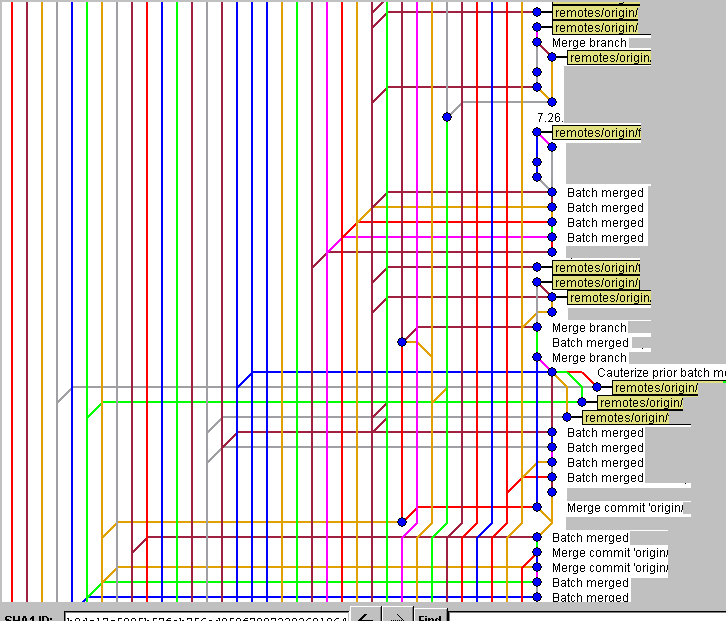
\includegraphics[width=75mm]{gitk.png}
        }
        \frame {
            \frametitle{git-gui - `a portable graphical interface to Git'}
            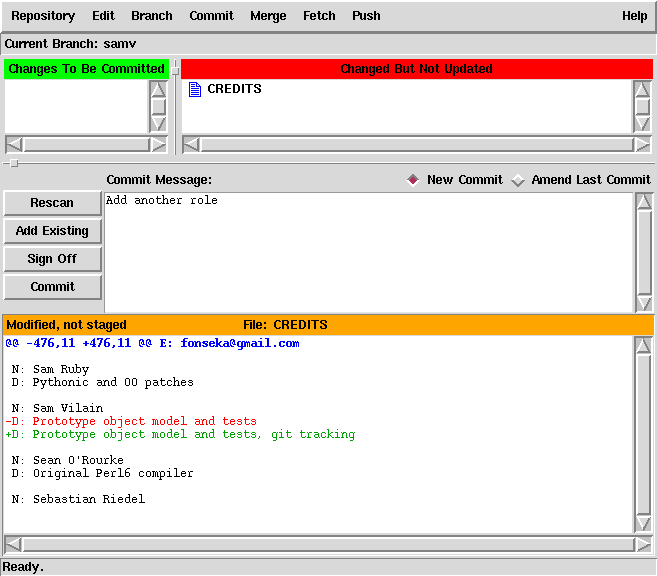
\includegraphics[width=75mm]{git-gui.png}
        }

    \subsection{Interacting with legacy tools}
        \frame {
            \frametitle{Importing from \$TOOL}

            \begin{itemize}
                \item Import complete history from:
                    \begin{itemize}
                        \item Subversion / SVK
                        \item CVS
                        \item Perforce
                        \item Mercurial
                        \item Darcs
                        \item Arch, Quilt, IBM Rational ClearCase, \ldots
                    \end{itemize}
                \item Roll your own imports easily with \lstinline!git-fast-import!.
                \item More info: 
                    \small{\url{http://git.or.cz/gitwiki/InterfacesFrontendsAndTools}}
            \end{itemize}
        }

        \frame {
            \frametitle{Working transparently with SVN repositories}

            \begin{itemize}
                \item Get:
                \begin{itemize}
                    \item The familiar, faster and saner Git tools
                    \item Off-line commits (whilst still being distributed)
                    \item The warm glow of elitism
                \end{itemize}
                \item More info: \lstinline!man git-svn!
            \end{itemize}
        }

    \subsection{Other stuff}
        \frame {
            \frametitle{Git-bisect}
            
            \begin{itemize}
                \item Useful for finding when a bug was introduced (which usually indicates how to fix the bug!)
                \item Binary searches revisions for fault
                \item Works by either:
                    \begin{itemize}
                        \item Manually specifying bad revisions (\lstinline!git bisect good/bad!)
                        \item Specifying a command that should be run on each revision
                    \end{itemize}
                \item Can be restricted to specified paths
                \item Most effective with good patch dicipline
            \end{itemize}
        }

        \frame {
            \frametitle{Current branch in shell prompt}
            
            \begin{itemize}
                \item Reduces repetitive typing of \lstinline!git branch!.
            \end{itemize}

            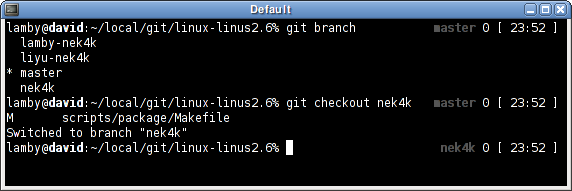
\includegraphics[width=110mm]{branch-prompt.png}
        }

%%%%%%%%%%%%%%%%%%%%%%%%%%%%%%%%%%%%%%%%%%%%%%%%%%%%%%%%%%%%%%%%%%%%%%%%%%%%%%%%%%%%%%%%%%

\frame {
    \frametitle{Thanks!}
    WUGLUG contact information:
    \begin{itemize}
        \item Website: \url{http://www.wuglug.org.uk}
        \item IRC: {\tt \#wuglug} on {\tt irc.uwcs.co.uk:6667}
        \item Mailing list: \url{https://www.warwickcompsoc.co.uk/mailman/listinfo/wuglug}
    \end{itemize}
}

\end{document}
